\chapter{Graphene monolayer}
We consider a tight-binding model in the Slater-Koster (SK) approximation with 4 orbitals for the $C$ atom ($s$,$p_x$,$p_y$,$p_z$) and 1 orbital ($s$) for the $H$ atom. The SK parameters used are:
\begin{equation}
  \begin{array}{l|cccc}
        & V_{ss\sigma} & V_{sp\sigma} & V_{pp\sigma} & V_{pp\pi} \\ \hline
    C-C & -7.76 & 8.16 & 7.48 & -2.7 \\
    C-H & -6.84 & 7.81 & \text{--} & \text{--}
  \end{array}\qquad\qquad
  \begin{array}{c|cccc}
    \text{On-site} & s & p_x & p_y & p_z \\ \hline
    C & -8.8 & 0.0 & 0.0 & 0.0 \\
    H & -2.5 &     &     &
  \end{array}
\label{SK_params}
\end{equation}

These parmeters are in line with those found in the literature\cite{Gosalbez-Martinez2011,Konschuh2010} and can be obtained by fitting of DFT bands (done with quantum-espresso). It is important to notice that the exact values for these parameters is not relevant since small deformation of them just result in small deformations of the band structure. The symmetries of graphene and its orbitals ensure that the components of the eigenstates are the correct ones since the $p_z$ is decoupled from all the other orbitals.

With these parameters we consider an armchair hexagonal nanoisland ($\sim10^4-10^5$ $C$ atoms). Such a system is 0-dimensional, hence, no band structure can be defined but rather just the spectrum. Nevertheless, in the limit of an infinite island, the physical properties of graphene should be recovered.
We can get an idea of how far from real graphene we are by considering the confinement gap. Graphene is famously known for not having a gap in the band structure. Graphene nanoislands do have a gap due to its finite size, but the larger the island, the smaller the gap until in the limit of an infinite island (graphene) the gap shall disappear. The dependence of the gap and the size of the island can be estimated as a free particle in a box of size $L$, roughly $\Delta\sim\frac{1}{L^2}$. Performing the actual calculation we can obtain see the dependence of the gap with the size of the island (see Fig.~\ref{confinement}) and estimate the necessary dimensions for our calculations.

%~~~~~~~~~~~~~~~~~~~~~~~~~~ FIGURE ~~~~~~~~~~~~~~~~~~~~~~~~~%
\begin{figure}[h!]
  \centering
  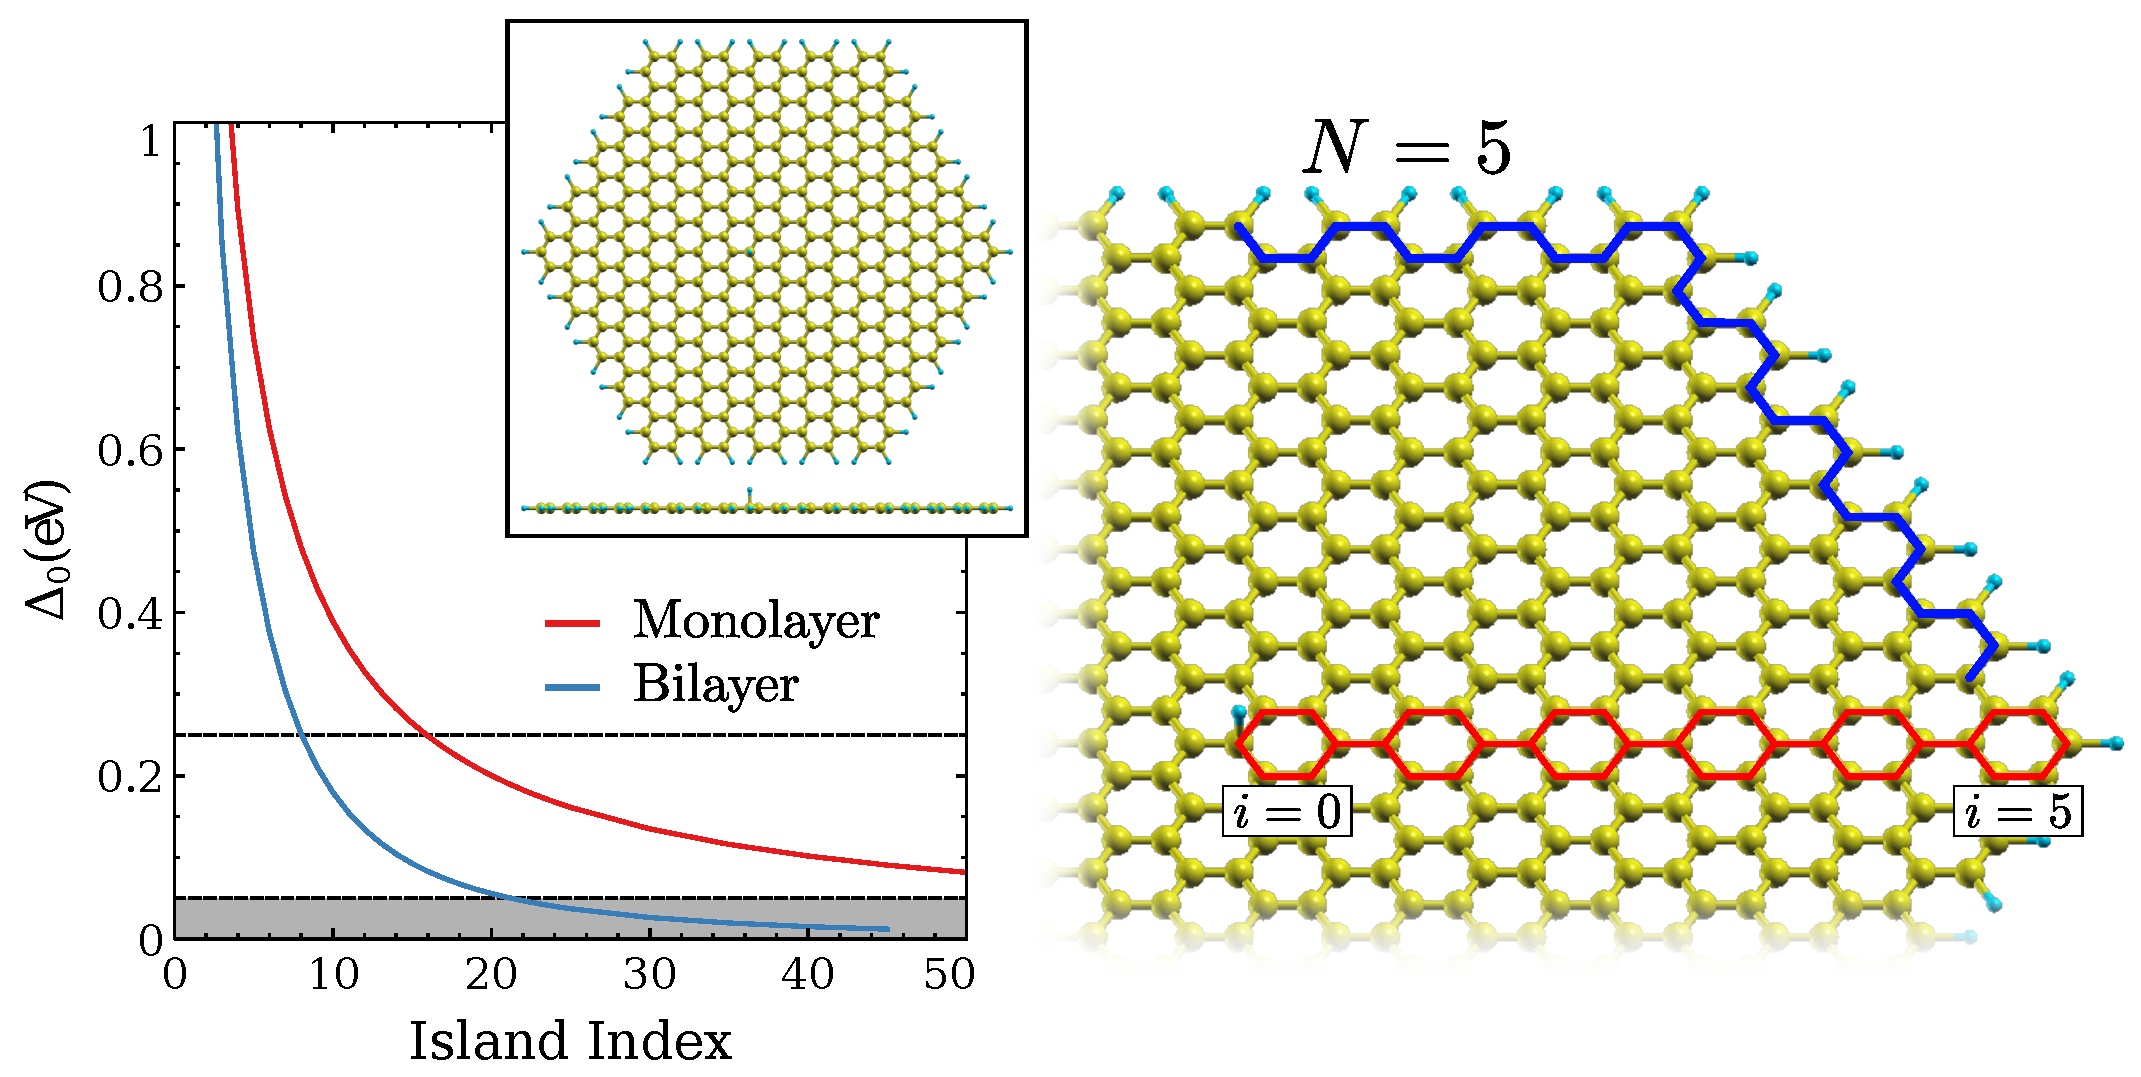
\includegraphics[width=0.9\textwidth]{defects/fig/cell.pdf}
  \vspace{-5pt}
\caption{Confinement gap for a monolayer and a bilayer of graphene. The island index labels the size of the island by the number of ``benzene blocks'' along the diagonal as shown in red in the right panel. The dashed line at $0.25eV$ corresponds to the largest gap opened bia electric gating in graphene bilayer\cite{Zhang2009}. We will consider the islands big enough to be considered as graphene when their confinement gap lies in the shadowed region.}
\label{confinement}
\end{figure}
% \FloatBarrier
%~~~~~~~~~~~~~~~~~~~~~~~~~~~~~~~~~~~~~~~~~~~~~~~~~~~~~~~~~~~%

When 4 orbitals are considered, the breaking of the $C_3$ symmetry at the edges (ie, the $C$ atoms in the edges are missing 1 neighbor) results in near-zero energy states due to the unmet $\sigma$ bonds, combination of $s$, $p_x$ and $p_y$. In order to get rid of these artificious states we consider the island edges to be pasivated by Hydrogen atoms as shown in Fig.~\ref{confinement}. This way the dangling bonds hybridize and get lifted/drowned to the $\sigma$ manifolds.
Although physically founded, the inclusion of $H$ pasivating atoms is somehow a technical construct to remove the dangling bonds from the low energy spectrum, hence, the strength of the $C-H$ bonds is not relevant and it should suffice to shift the $\sigma$ states far away from the low energy part of the spectrum.

% Such parameters yield the following band structure for graphene
\section{H adatom on graphene monolayer}
When a Hydrogen atom is placed on top of one of the $C$ atoms of graphene, the $s$ orbital of the Hydrogen hybridizes with both the $s$ and the $p_z$ orbitals of the Carbon. All the other hoppings are strictly zero due to the symmetry and disposition of the orbitals.

The general understanding is that a $H$ adatom on graphene can be understood as a vacancy in the $p_z$ subspace. The reason for this is that the $s$ orbital of the $H$ hybridizes with the $s$ and $p_z$ orbitals of the $C$ atom (all other hoppings vanish because of symmetry). In the scenario of a vacancy in the $p_z$ manifold, the system is exactly a bipartite lattice, and following (one of) the Lieb's theorems, the imbalance in the number of atoms in one of the sublattices results in zero energy states.

The Lieb's Theorem holds for bipartite lattices at half filling, which is indeed the case of graphene when only $p_z$ orbitals are considered. The inclusion of the other $p$ orbitals does not break the bipartite nature of the lattice since their manifold is disconnected from that of the $p_z$ orbitals, \emph{and their on-site energy is the same}.
The $s$ orbitals are also disconnected from the $p_z$ manifold but their on-site energy is different from zero (see \ref{SK_params}). This fact breaks the bipartite character of the lattice, nevertheless, the $s$ manifold is far in energy and its hybridization with the $p_{x/y}$ orbitals is strong so the bonding-antibonding states are also far in energy.

It is instructive to compare the spectrum of a big armchair island (22686 $C$ atoms) considering 4 orbitals and a $H$ adatom and the same island with only $p_z$ orbitals and a vacancy.

%~~~~~~~~~~~~~~~~~~~~~~~~~~ FIGURE ~~~~~~~~~~~~~~~~~~~~~~~~~%
\begin{figure}[h!]
  \centering
  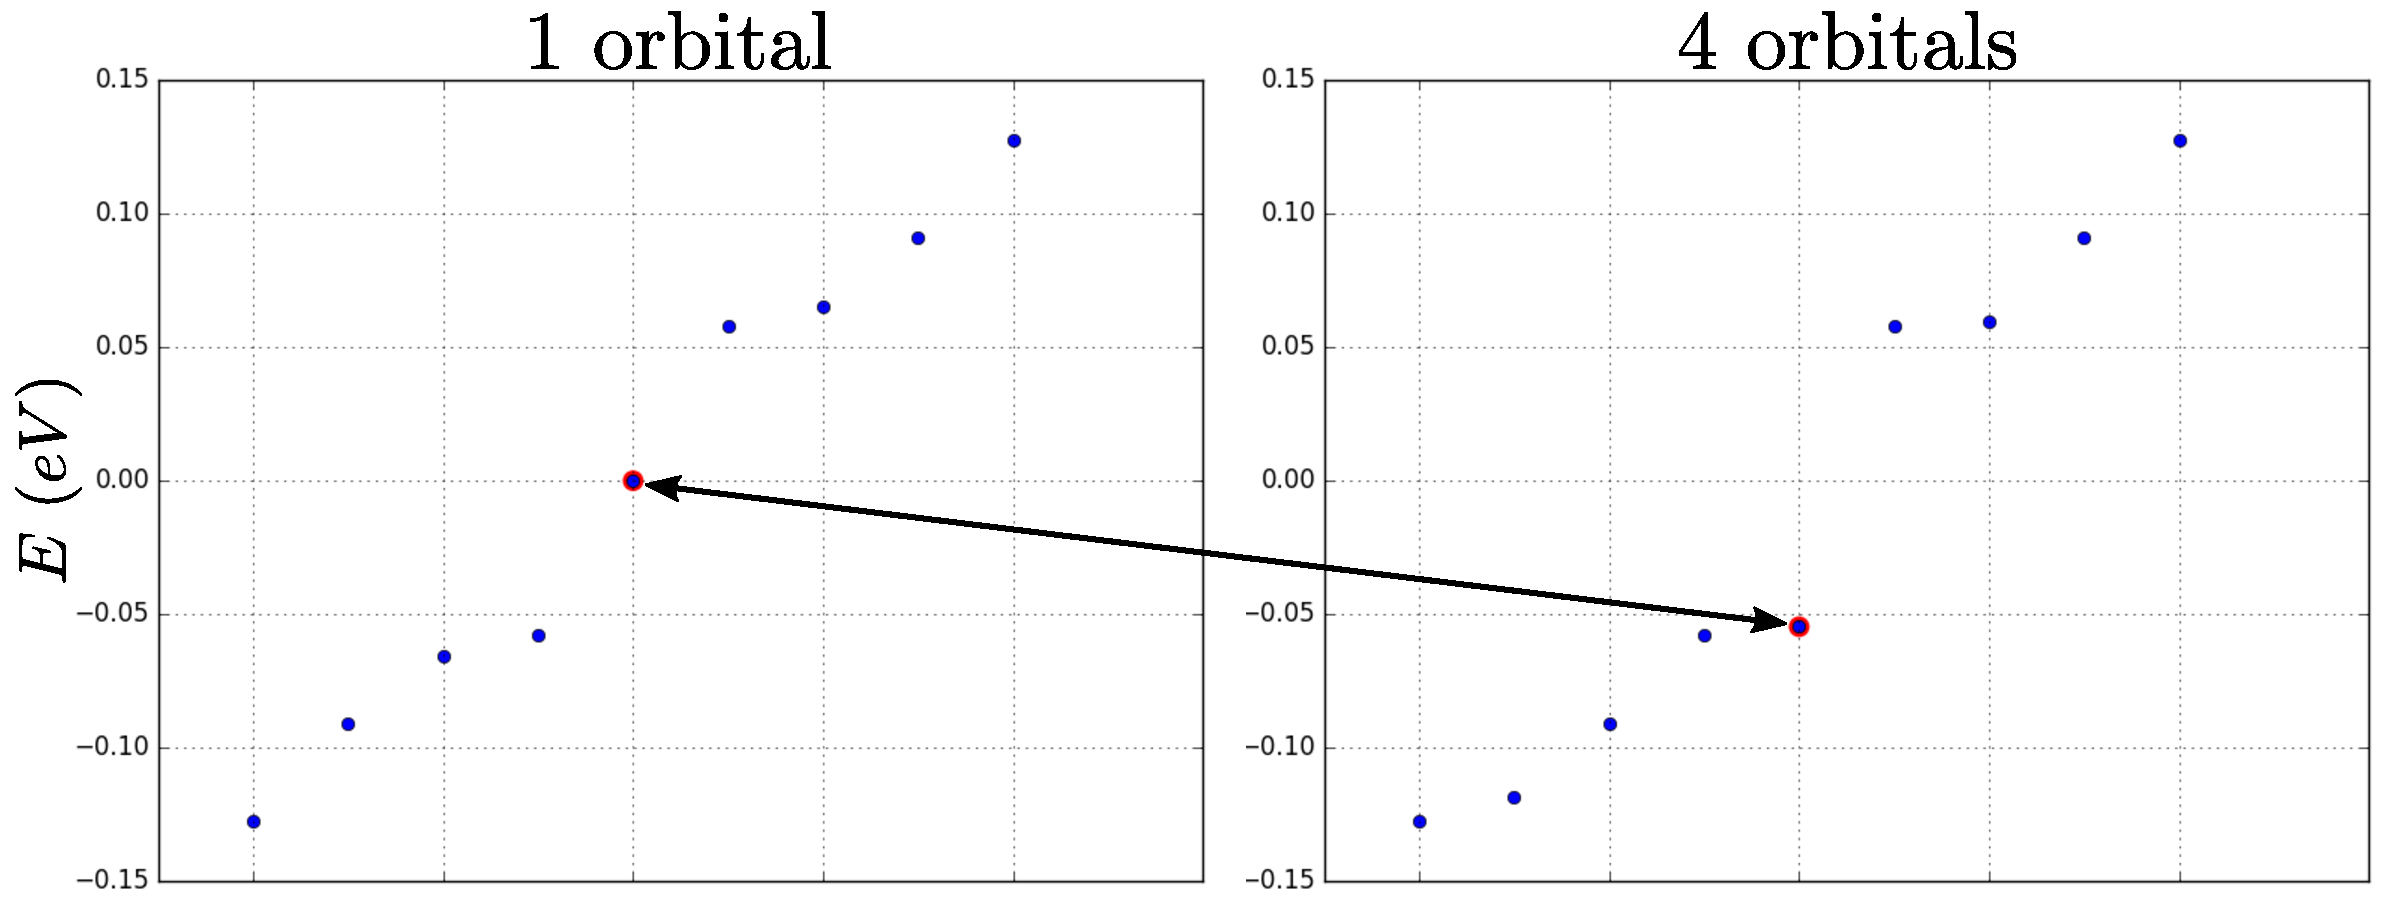
\includegraphics[width=0.8\textwidth]{defects/fig/spectrum.pdf}
  \vspace{-5pt}
\caption{Low energy spectrum of an armchair island. Left panel shows the spectrum when only the $p_z$ orbitals are considered. Right panel shows the spectrum considering all 4 orbitals $s$, $p_x$, $p_y$, $p_z$}
\label{spectrum}
\end{figure}
\FloatBarrier
%~~~~~~~~~~~~~~~~~~~~~~~~~~~~~~~~~~~~~~~~~~~~~~~~~~~~~~~~~~~%

Notice in figure~\ref{spectrum} that the in-gap state, marked in red, does not appear at $E=0$ as this system is no longer suitable for the Lieb's theorem. The exact energy at which the in-gap state appear depends on the hopping parameters between the $H$ and the $C$ atoms, mainly on the $V_{sp\sigma}$ parameter.

The parameters in \ref{SK_params} were calculated for $H$ pasivating the edges of graphene nanoribbons where the main hybridization occurs with the $\sigma$ orbitals of graphene. There is no good reason why these hoppings parameters should hold for an adatom, so we can consider the hopping parameters, $V_{ss\sigma}$ and $V_{sp\sigma}$, between the chemisorbed Hydrogen and graphene as somehow free parameters that we can tune.

The position of the in-gap state as a function of both parameters is shown in fig~\ref{ingap}. Notice the strong dependence with the $V_sp\sigma$ parameter.
%~~~~~~~~~~~~~~~~~~~~~~~~~~ FIGURE ~~~~~~~~~~~~~~~~~~~~~~~~~%
\begin{figure}[h!]
  \centering
  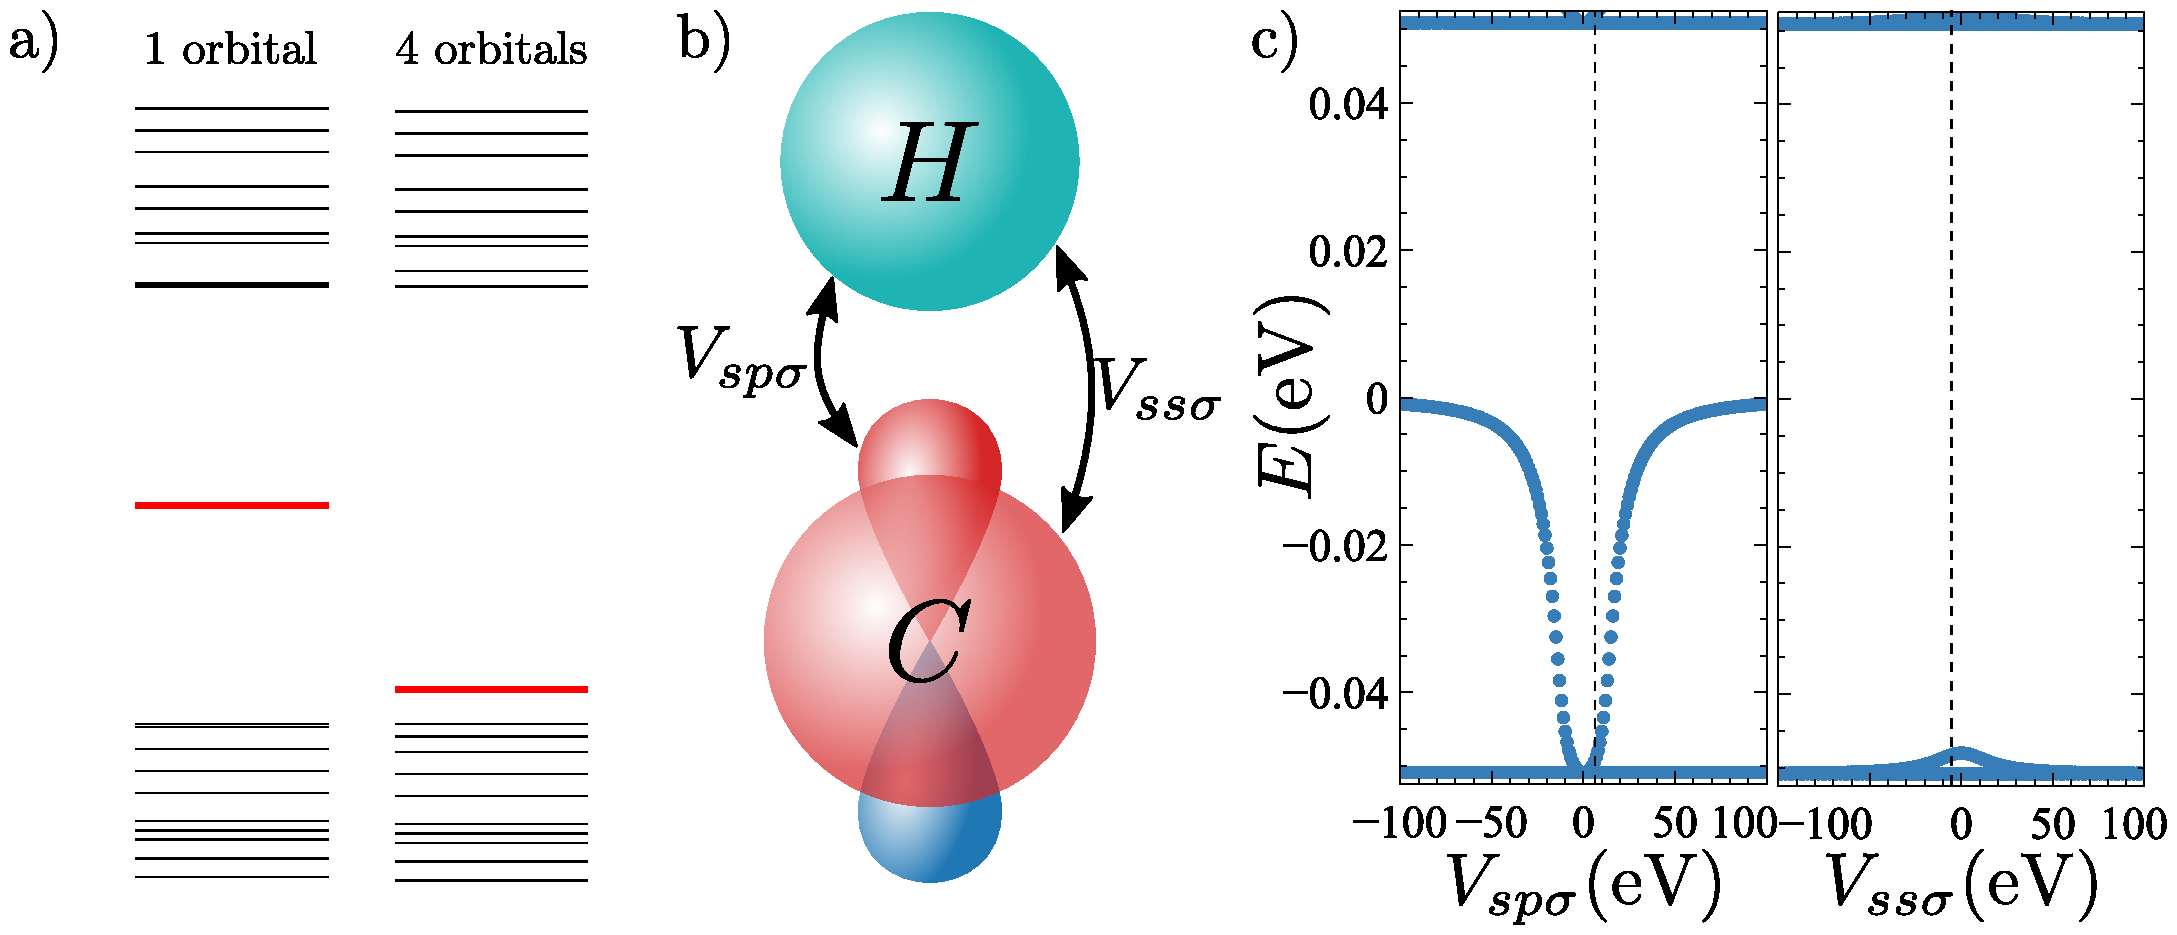
\includegraphics[width=0.8\textwidth]{defects/fig/Vsss_Vsps.pdf}
  \vspace{-5pt}
\caption{Position of the in-gap state of an adatom on a graphene nanoisland as a function of the hopping parmeters $V_{sp\sigma}$ and $V_{ss\sigma}$. In the plot the whole range to $\pm\infty$ is explored although the relevant part is only around 0, namely [-20,20].}
\label{ingap}
\end{figure}
\FloatBarrier
%~~~~~~~~~~~~~~~~~~~~~~~~~~~~~~~~~~~~~~~~~~~~~~~~~~~~~~~~~~~%
It is clear that in order to recover the 1 orbital intuition (in-gap state at $E=0$), we require the limit for $V_{sp\sigma}\to\infty$. The experimental value for these parameters is difficult to infer, so we will consider a wide range of value and explore the resulting physics.

We start by plotting the position of the in-gap state and the hyperfine coupling  as a function of the two parameters


%~~~~~~~~~~~~~~~~~~~~~~~~~~ FIGURE ~~~~~~~~~~~~~~~~~~~~~~~~~%
\begin{figure}[h!]
  \centering
  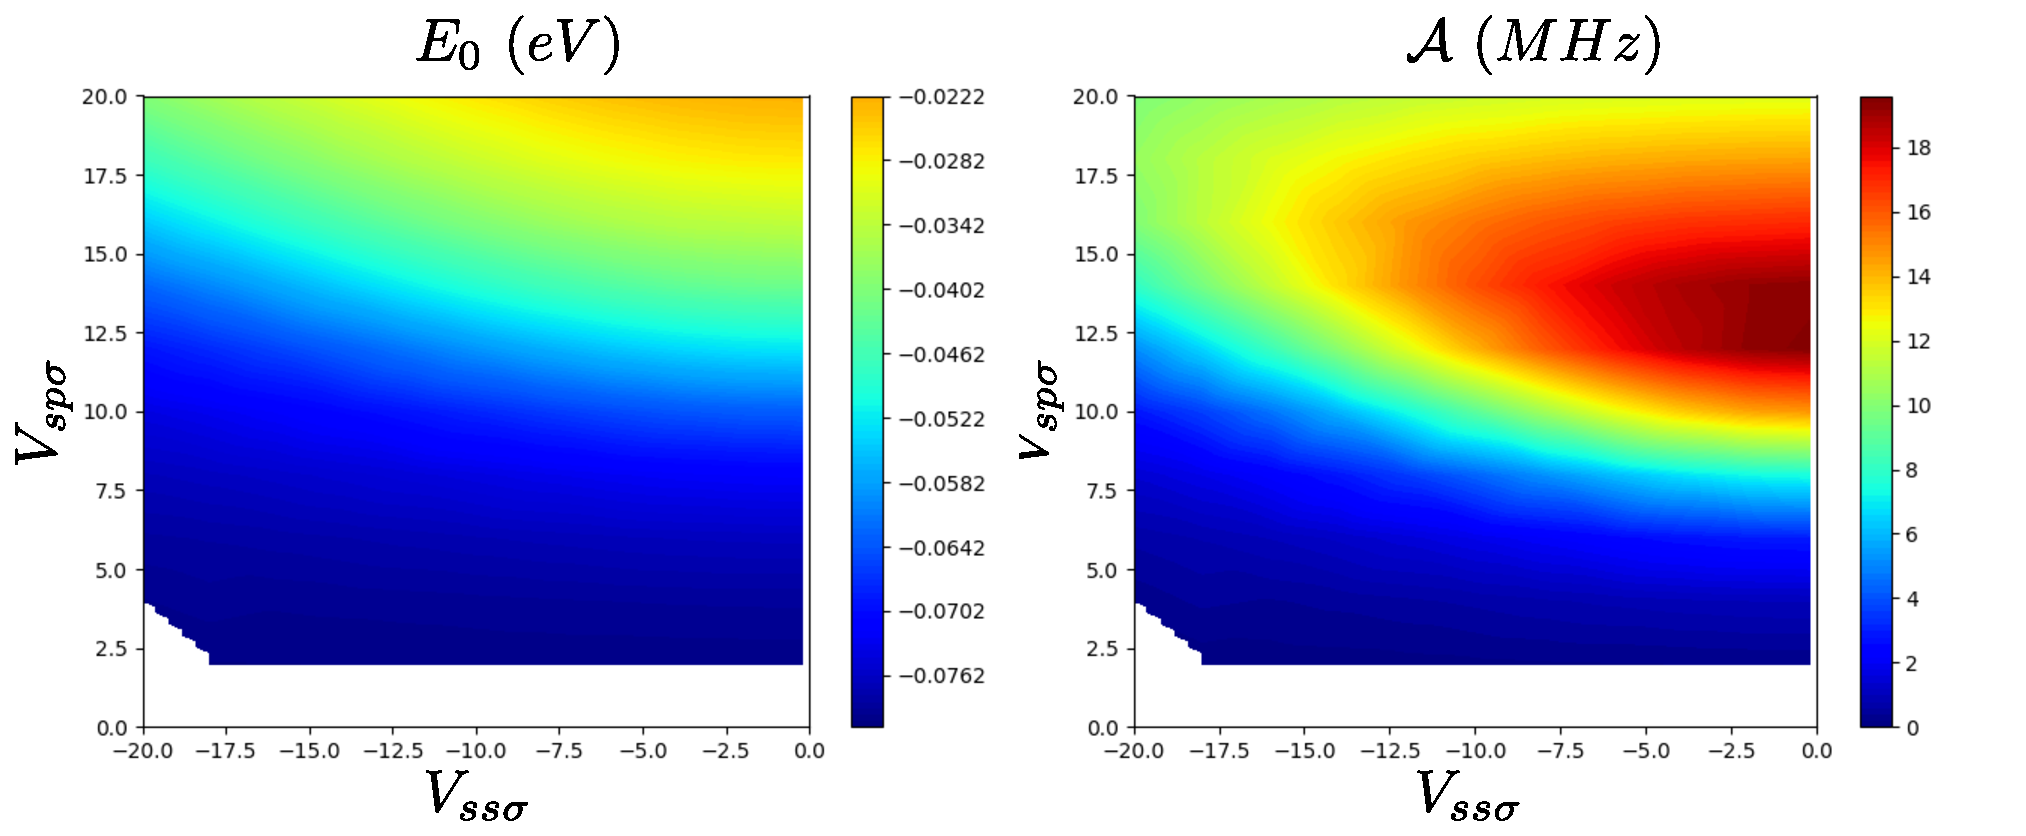
\includegraphics[width=0.9\textwidth]{defects/fig/parameter_space_mono.pdf}
  \vspace{-5pt}
\caption{Parameter space for the energy of the in-gap state and the hyperfine coupling for a graphene nanoisland.}
\label{SK2d}
\end{figure}
\FloatBarrier
%~~~~~~~~~~~~~~~~~~~~~~~~~~~~~~~~~~~~~~~~~~~~~~~~~~~~~~~~~~~%







\section{Graphene bilayer}
Graphene bilayer can be described in a analogously. The interlayer hopping is estimated by scaling down the parameters \eqref{SK_params} by a factor, $\xi$, such that the $p_z-p_z$ interlayer hopping takes a value\cite{KatsnelsonBook} of $\xi t_{p_z-p_z}\simeq 0.4eV$.
% Fig~\ref{hoppings} shows all the possible hoppings between two C atoms in different layers. It is important to notice that in the case of graphene bilayer, the $p_z$ manifold is no longer decoupled from the rest of the orbitals as in the case of graphene.
% %~~~~~~~~~~~~~~~~~~~~~~~~~~ FIGURE ~~~~~~~~~~~~~~~~~~~~~~~~~%
% \begin{figure}[h!]
% \centering
%   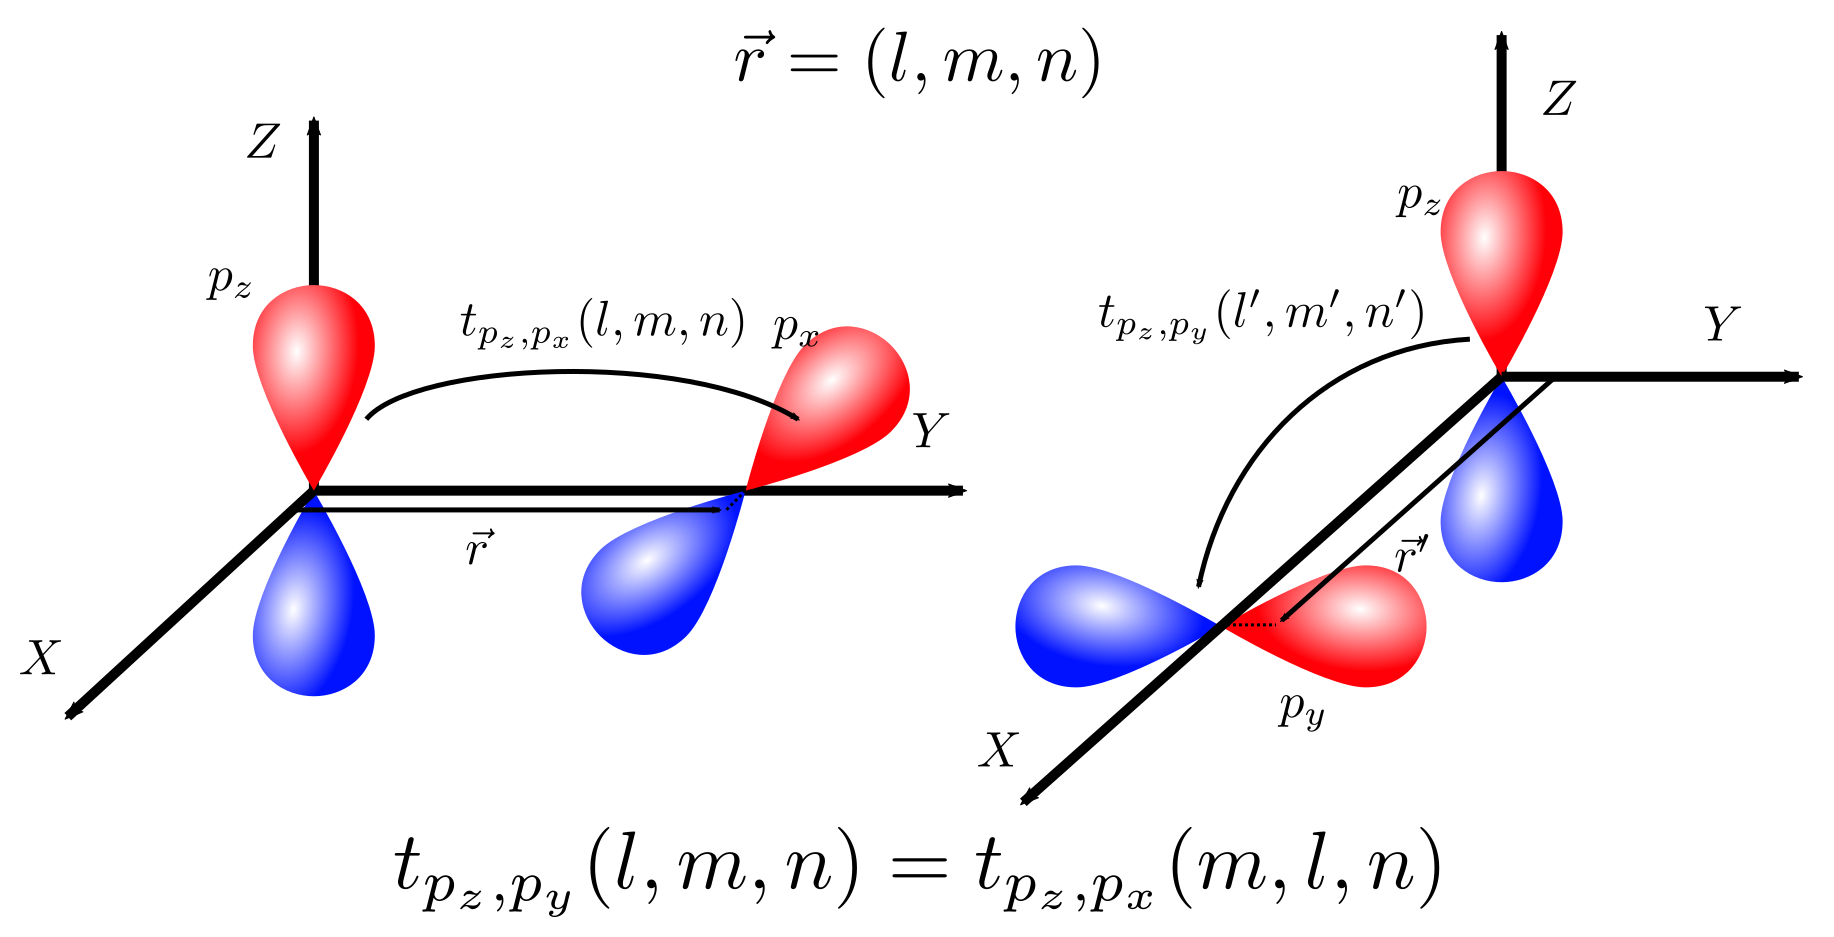
\includegraphics[width=0.45\textwidth]{SK.pdf}
%   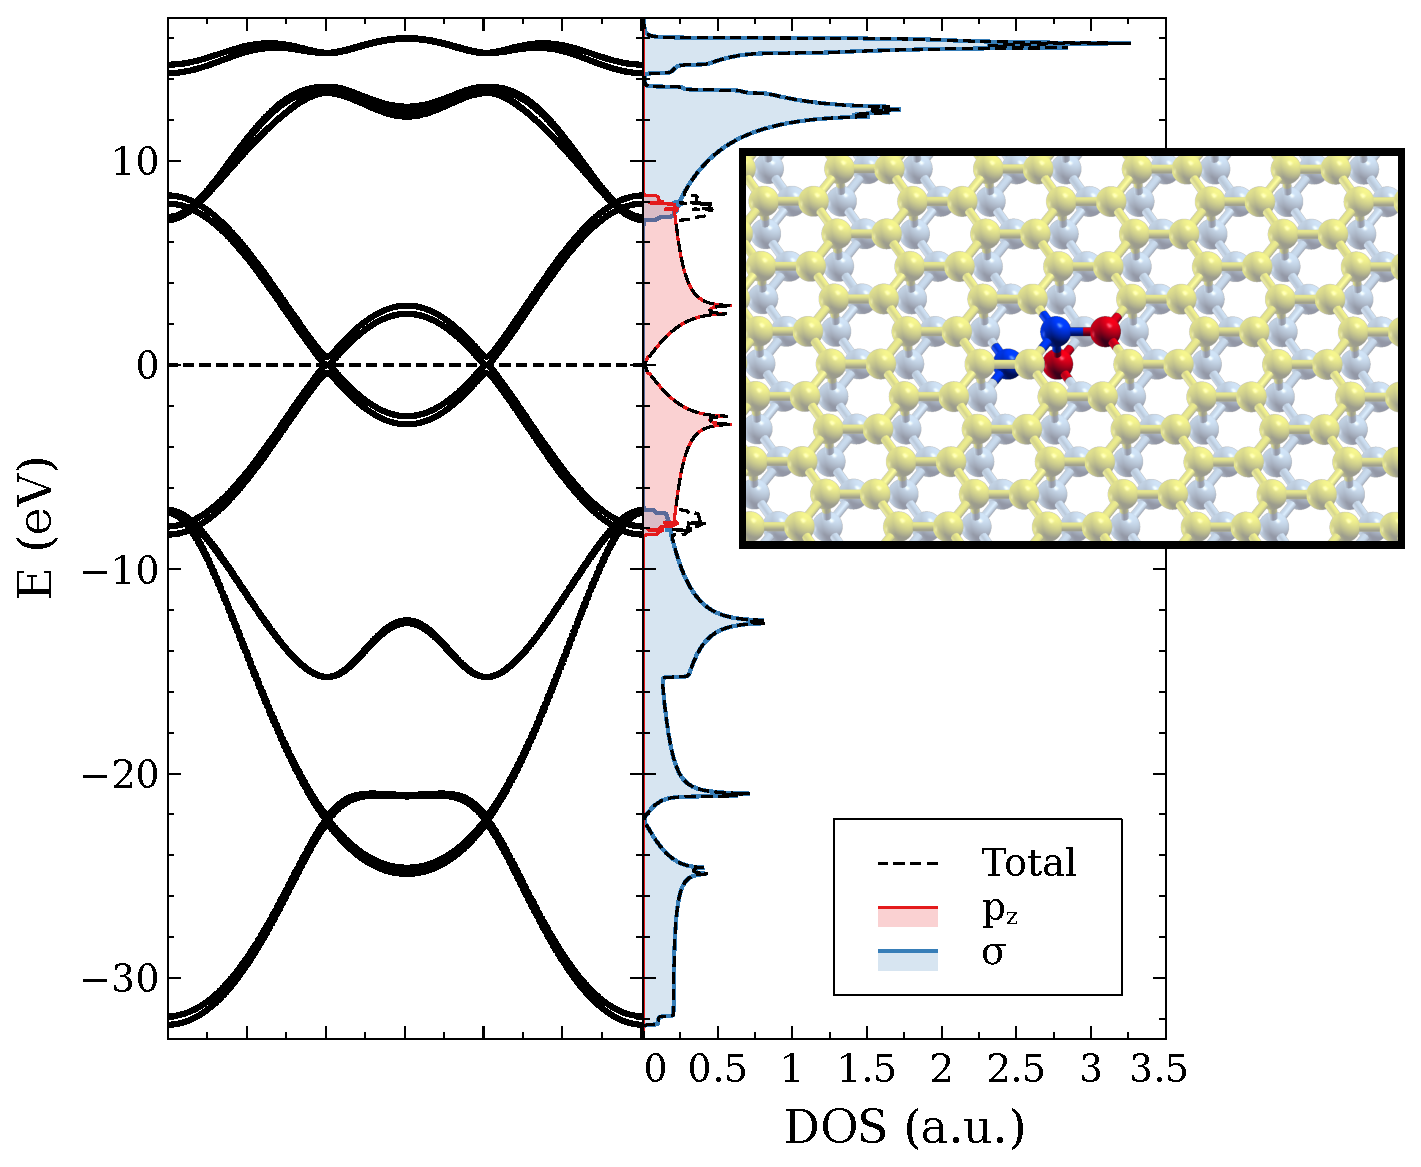
\includegraphics[width=0.45\textwidth]{bilayer_bandDOS.pdf}
% \vspace{-5pt}
% \caption{a) Panel show All the possible interlayer hoppings in graphene bilayer. b) Band structure and density of states of graphene bilayer}
% \label{hoppings}
% \end{figure}
% \FloatBarrier
% %~~~~~~~~~~~~~~~~~~~~~~~~~~~~~~~~~~~~~~~~~~~~~~~~~~~~~~~~~~~%
\subsection{Electric field}
% The band structure of graphene bilayer in such a model is shown in \ref{hoppings}.
The effect of an electric, $\Delta_E$ is to shift the energies of all the orbitals by an amount $\pm\Delta_E$, depending on the layer. This shift opens a gap in the Dirac Points. In nanoislands it can be seen that the gap opens linearly (for low field) with the electric field.

%~~~~~~~~~~~~~~~~~~~~~~~~~~ FIGURE ~~~~~~~~~~~~~~~~~~~~~~~~~%
\begin{figure}[h!]
  \centering
  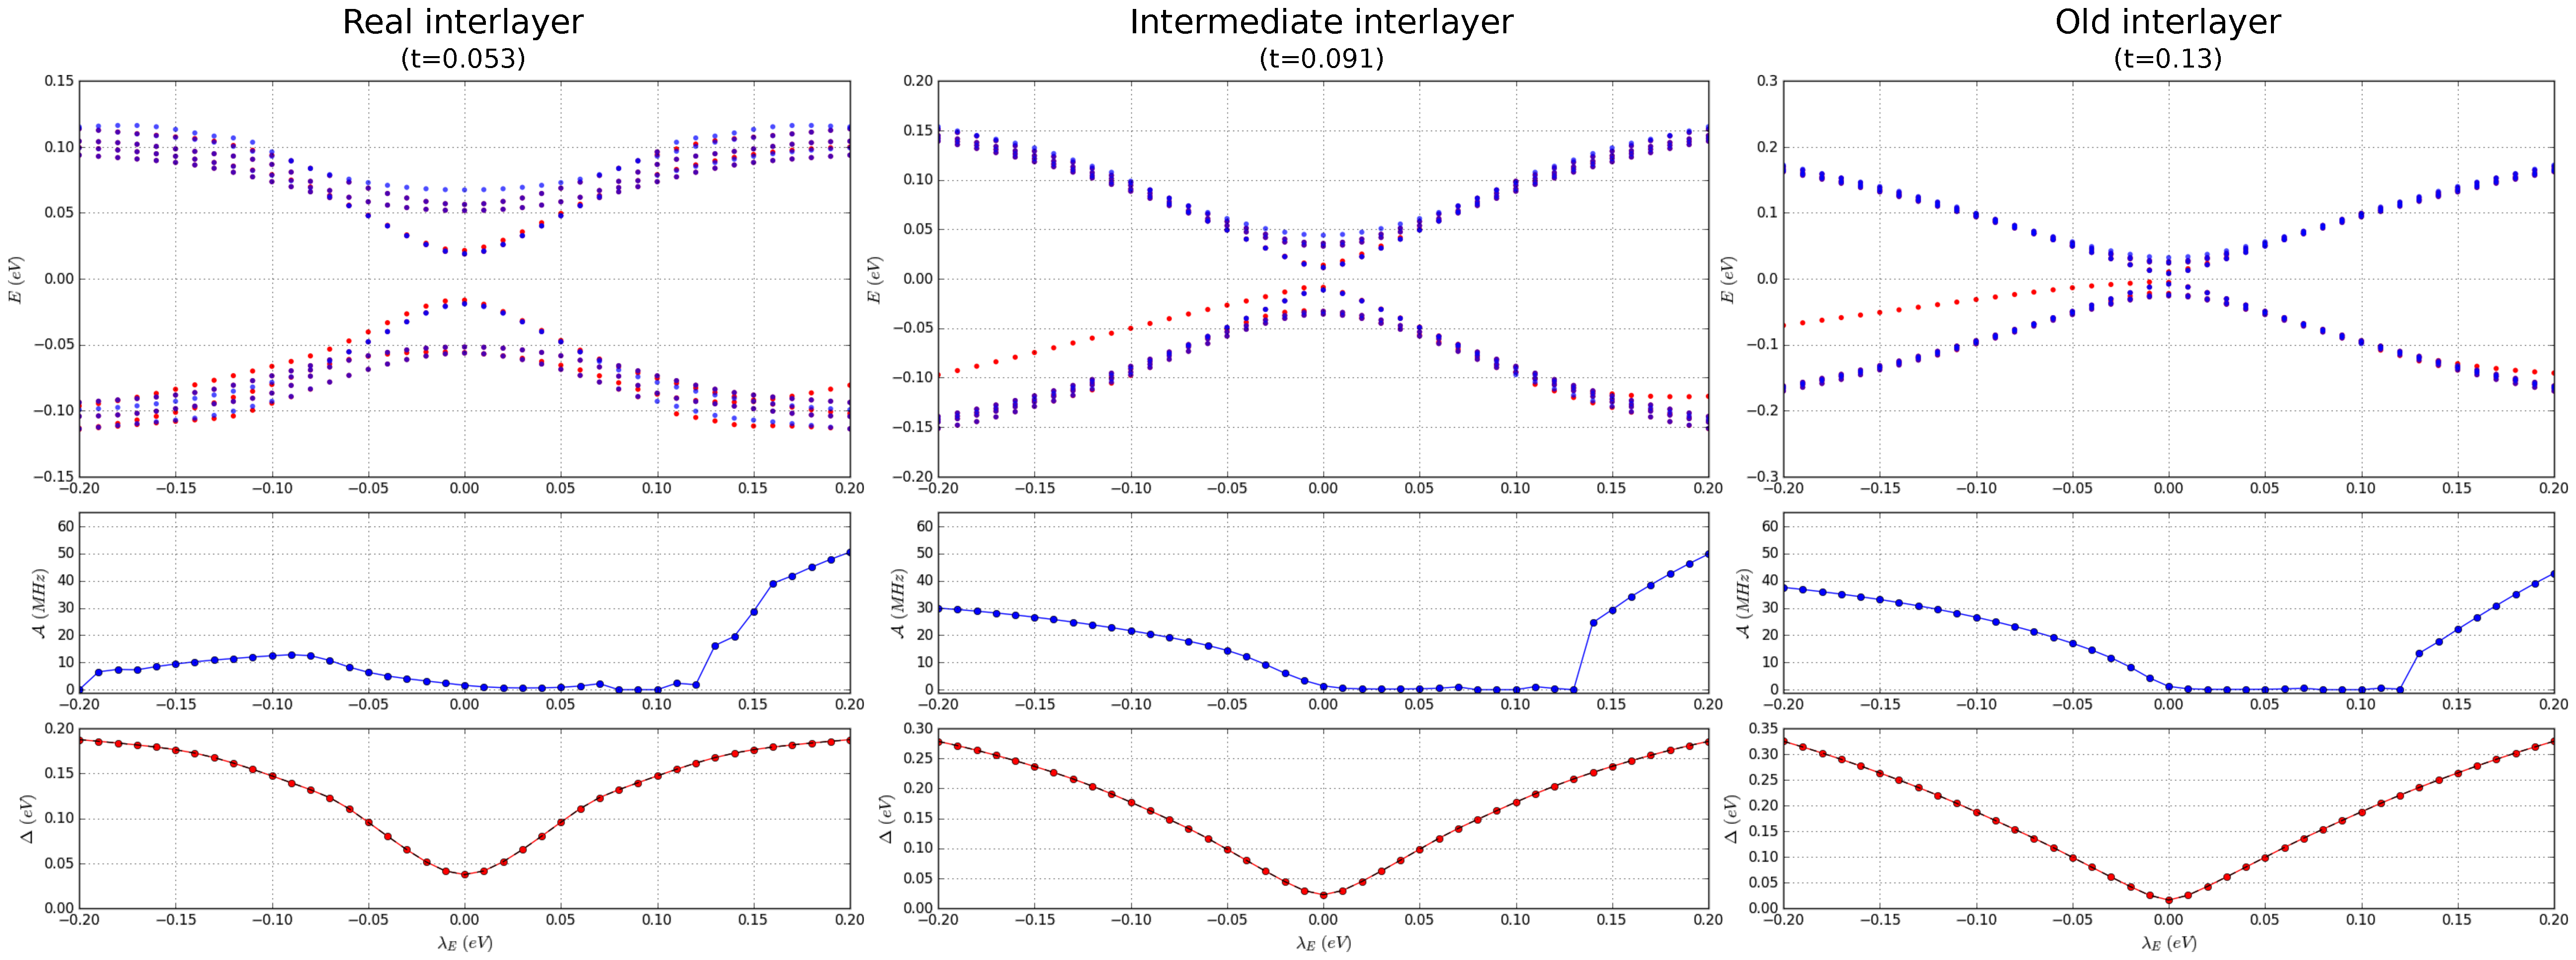
\includegraphics[width=\textwidth]{defects/fig/interlayer_elec.pdf}
  \vspace{-5pt}
\caption{Evolution of the low energy spectrum (the 8 eigenvalues closest to $E=0$), the hyperfine coupling and the gap with the electric field for different interlayer couplings. In the first panels the blue dots are the spectrum for the pristine island, without $H$ adatom and the red one is the defected case.}
\label{spectrums}
\end{figure}
\FloatBarrier
%~~~~~~~~~~~~~~~~~~~~~~~~~~~~~~~~~~~~~~~~~~~~~~~~~~~~~~~~~~~%

Given an island of a certain size (within the shadowed region in Fig.~\ref{confinement}) the evolution of the spectrum is shown in Fig.~\ref{spectrums}, Notice that the figure \emph{does not show bands} but rather discrete spectrums at different electric fields, in particular, the point at $\Delta_E=0$ \emph{is not the Dirac point}, it is simply the spectrum at zero electric field.

The main information that we can extract by now from Fig.~\ref{spectrums} is that the electronic structure of graphene bilayer opens a gap with the electric field.

The real value of the interlayer should be the one in the left panel, and it will be the one used from now on, meaning that \emph{the interlayer coupling will not be a free parameter in our calculations}.


\section{H adatom on graphene bilayer}

The physics of a $H$ adatom on bilayer graphene does not differ much from the monolayer case. In this case, again the Lieb's theorem nearly applies, although not exactly since the presence of $s$ orbitals break the bipartite character of the system.

To strictly recover the vacancy limit we would need to freeze the $s-s$ hopping ($V_{ss\sigma}\to0$) and increase the $s-p_z$ ($V_{sp\sigma}\to\infty$) as well as the on-site of the H atom ($\varepsilon_{H_s}\to-\infty$).

The effect of having finite hoppings and on-site energy is that the ``zero energy'' state is no longer at $E=0$.

%~~~~~~~~~~~~~~~~~~~~~~~~~~ FIGURE ~~~~~~~~~~~~~~~~~~~~~~~~~%
\begin{figure}[h!]
  \centering
  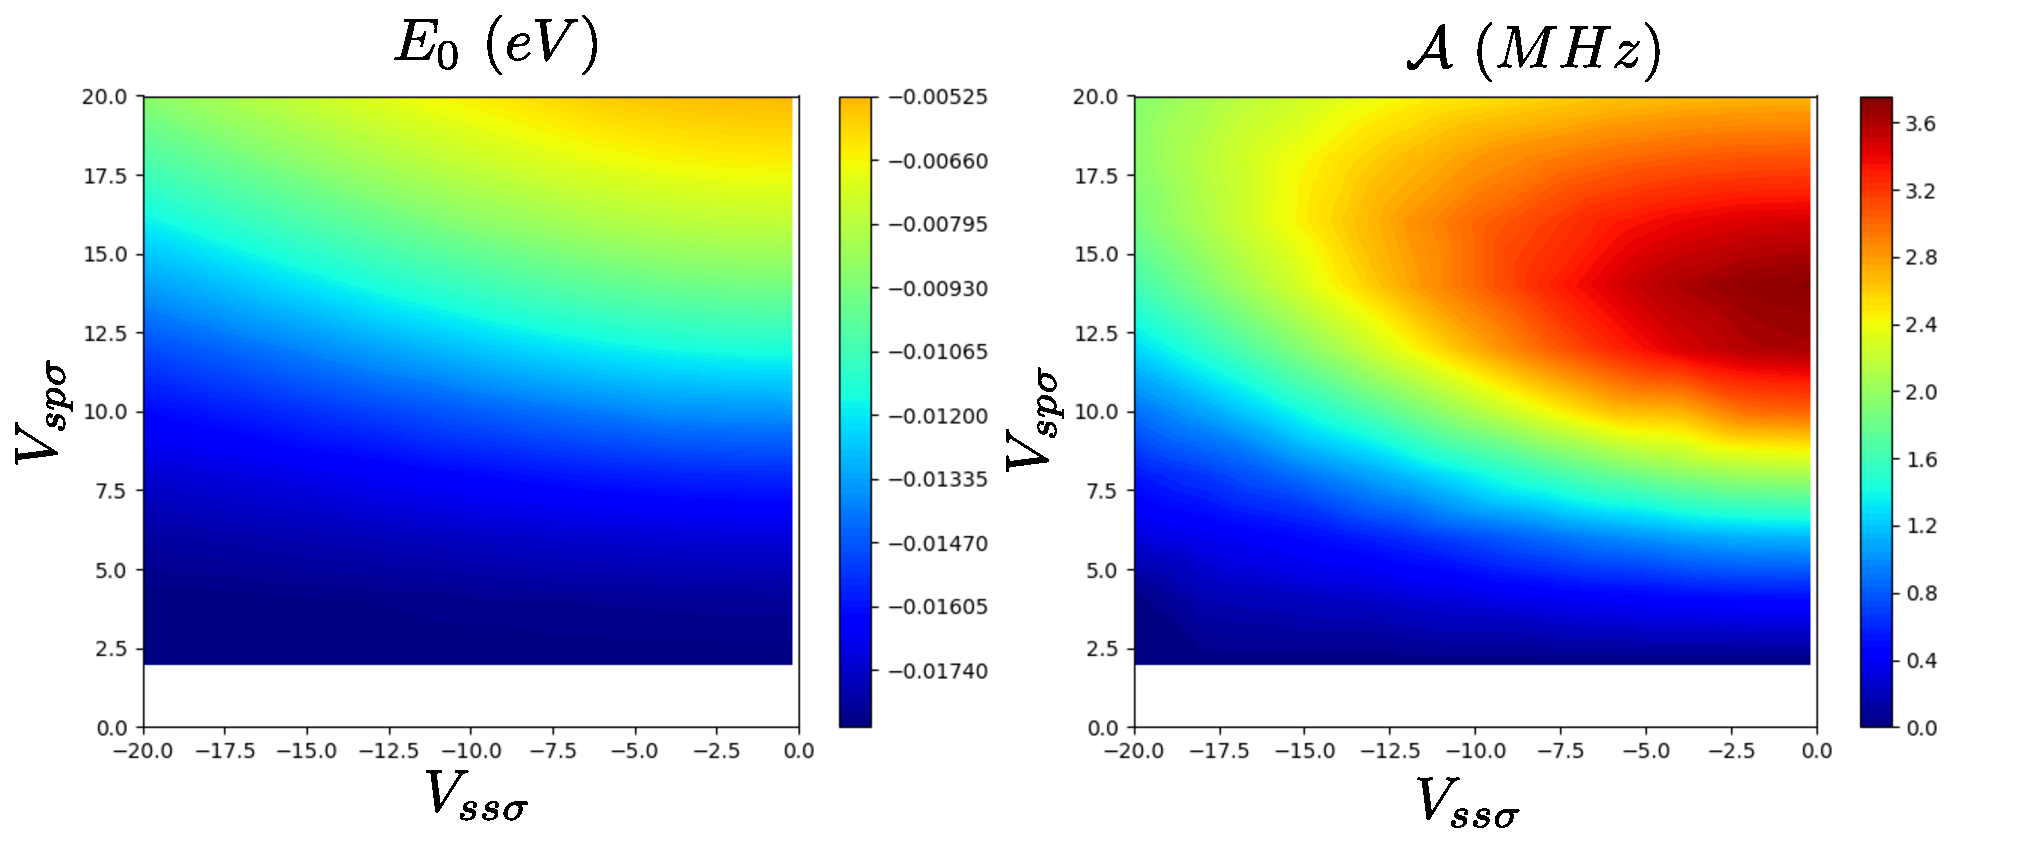
\includegraphics[width=0.9\textwidth]{defects/fig/parameter_space_bi.pdf}
  \vspace{-5pt}
\caption{Parameter space for the energy of the in-gap state and the hyperfine coupling for a graphene bilayer nanoisland.}
\label{SK2d_bi}
\end{figure}
\FloatBarrier
%~~~~~~~~~~~~~~~~~~~~~~~~~~~~~~~~~~~~~~~~~~~~~~~~~~~~~~~~~~~%

Notice that the parameter space $V_{ss\sigma}-V_{sp\sigma}$ looks quite similar to the monolayer case (Fig.~\ref{SK2d}) although there is a strong reduction in the hyperfine coupling $\mathcal{A}$ since the in-gap state is extended now among roughly twice as many atoms.\\


Choosing a value of  $V_{ss\sigma}$, $V_{sp\sigma}$ in the higest region in Fig.~\ref{SK2d_bi} we can see the evolution with the electric field:
%~~~~~~~~~~~~~~~~~~~~~~~~~~ FIGURE ~~~~~~~~~~~~~~~~~~~~~~~~~%
\begin{figure}[h!]
  \centering
  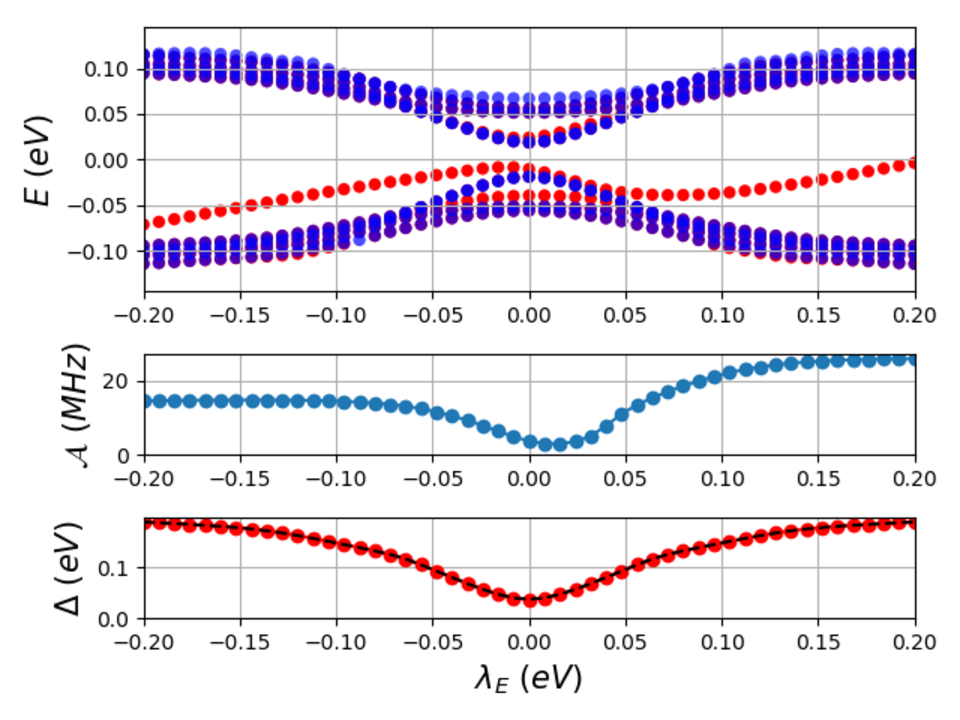
\includegraphics[width=0.6\textwidth]{defects/fig/best.pdf}
  \vspace{-5pt}
\caption{Evolution of the 8 eigenstates closest to $E=0$, the hyperfine coupling and the gap with the electric field}
\label{best}
\end{figure}
\FloatBarrier
%~~~~~~~~~~~~~~~~~~~~~~~~~~~~~~~~~~~~~~~~~~~~~~~~~~~~~~~~~~~%


And this is what the hyperfine coupling looks like in the parameter space $V_{ss\sigma}-V_{sp\sigma}$ when the electric field is switched on:
%~~~~~~~~~~~~~~~~~~~~~~~~~~ FIGURE ~~~~~~~~~~~~~~~~~~~~~~~~~%
\begin{figure}[h!]
  \centering
  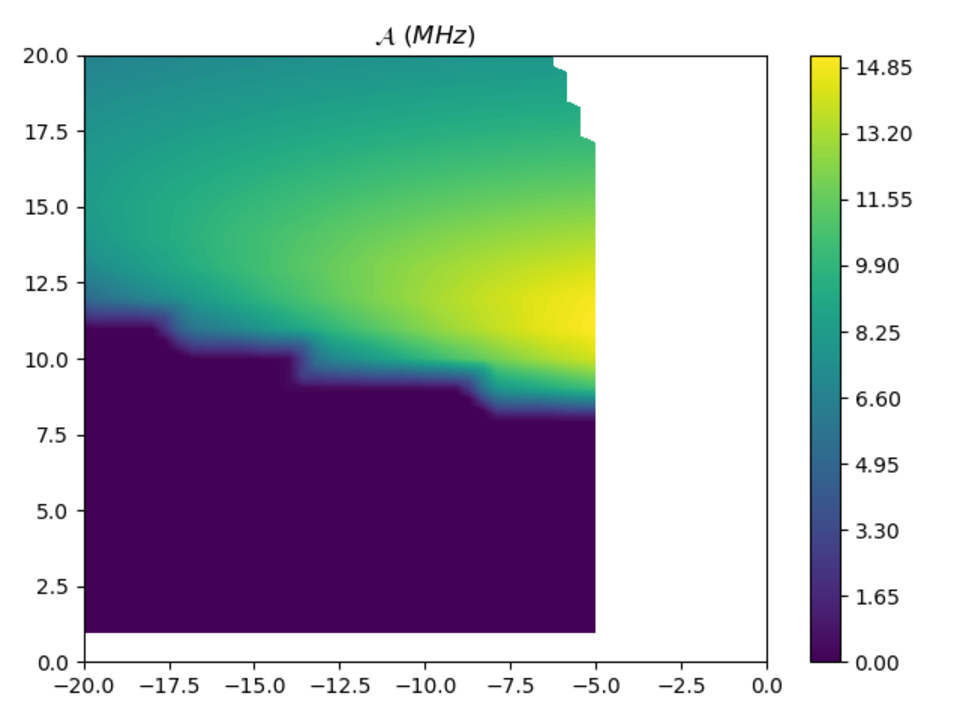
\includegraphics[width=0.6\textwidth]{defects/fig/SK_A_bi_e-02.pdf}
  \vspace{-5pt}
\caption{Parameter space for the hyperfine coupling for a graphene bilayer nanoisland in the presence of a strong electric field $\Delta_E=-0.2eV$}
\end{figure}
\FloatBarrier
%~~~~~~~~~~~~~~~~~~~~~~~~~~~~~~~~~~~~~~~~~~~~~~~~~~~~~~~~~~~%
